\input{../../doc}
\input{../../preamb}
\geometry{verbose,a4paper, inner=1cm, outer=1 cm, bmargin=2cm, tmargin=1cm}
\begin{document}
\pagestyle{empty}
\large
\begin{enumerate}
	\item Bruk eit og eit 100 kvadrat (snu arket) til å fargelegge alle tala i 2-gongen, 3-gongen og så videre opp til 11-gongen. (Eit tal som 90 er også i 2-gongen, sidan $2\cdot45=90$). Diskuter mønstra som dukker opp.
	\item Sjå på figur a). Kvifor er det rett å seie at den viser alle gongestykka du treng å vite for å kunne den lille gongetabellen?
	\item Sjå på figur b). Er det nokre av dei merka tala som ein finn igjen på dei fargelagde 100 kvadrata? Kva kallar vi desse tala?
\end{enumerate}
\begin{center}
	a) 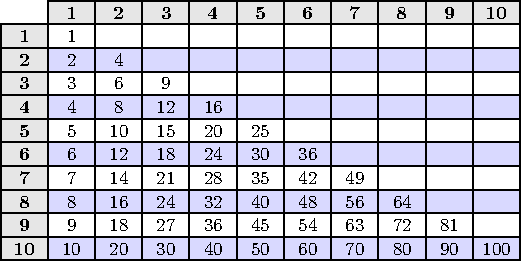
\includegraphics{smalltimestable} \qquad b) 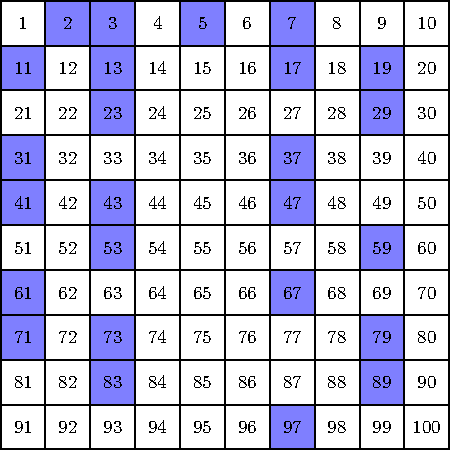
\includegraphics{primn100}
\end{center}
\newpage
\begin{center}
	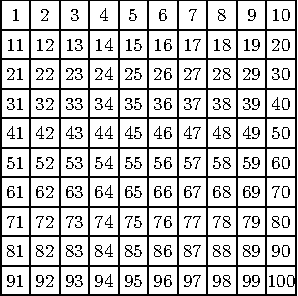
\includegraphics{100ark} \qquad \qquad
	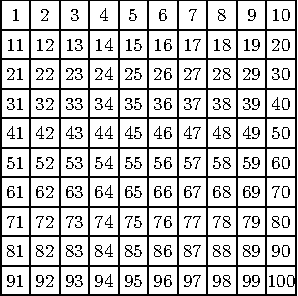
\includegraphics{100ark}
\end{center}
\begin{center}
	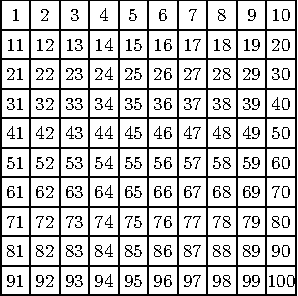
\includegraphics{100ark} \qquad \qquad
	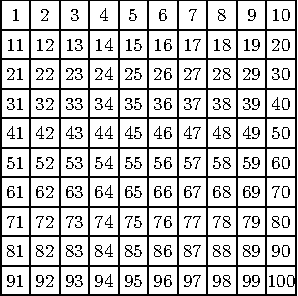
\includegraphics{100ark}
\end{center}
\begin{center}
	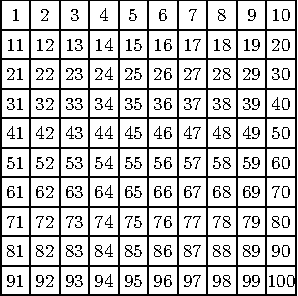
\includegraphics{100ark} \qquad \qquad
	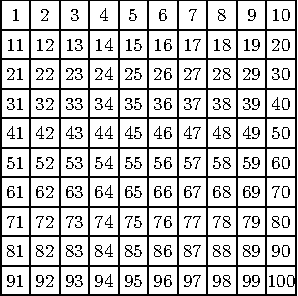
\includegraphics{100ark}
\end{center}
\begin{center}
	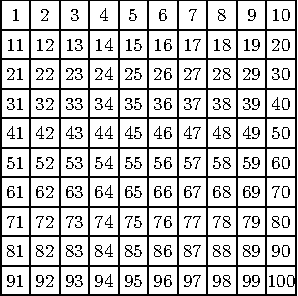
\includegraphics{100ark} \qquad \qquad
	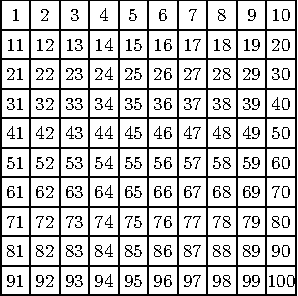
\includegraphics{100ark}
\end{center}
\begin{center}
	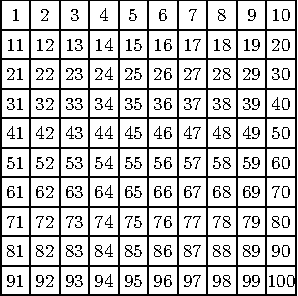
\includegraphics{100ark} \qquad \qquad
	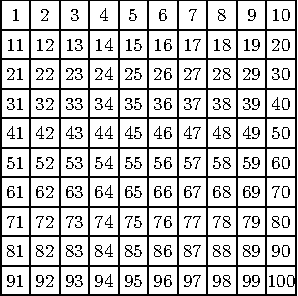
\includegraphics{100ark}
\end{center}
\newpage
\begin{center}
	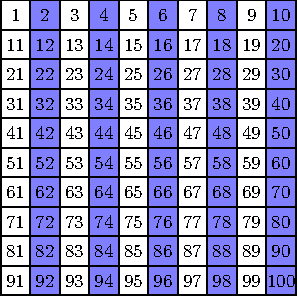
\includegraphics{2} \qquad \qquad
	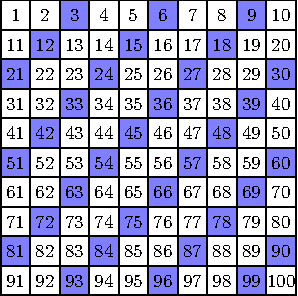
\includegraphics{3}
\end{center}
\begin{center}
	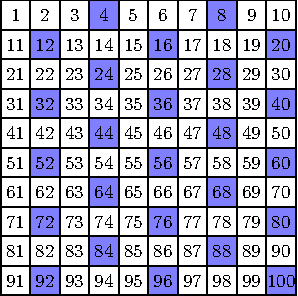
\includegraphics{4} \qquad \qquad
	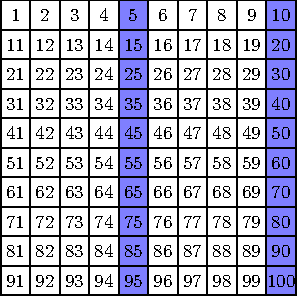
\includegraphics{5}
\end{center}
\begin{center}
	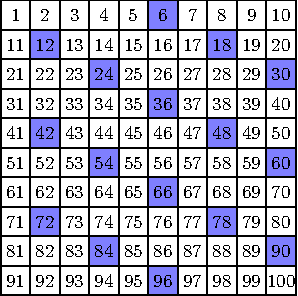
\includegraphics{6} \qquad \qquad
	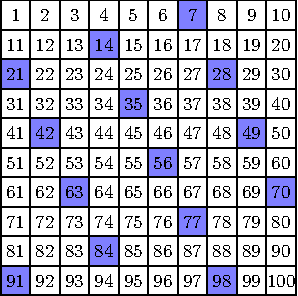
\includegraphics{7}
\end{center}
\begin{center}
	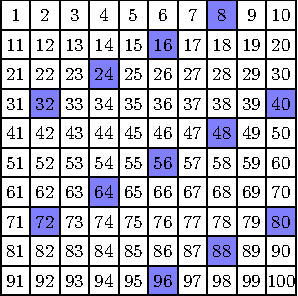
\includegraphics{8} \qquad \qquad
	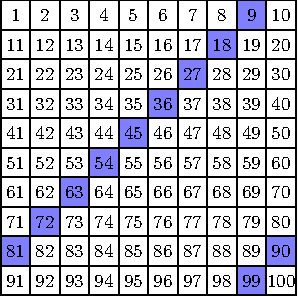
\includegraphics{9}
\end{center}
\begin{center}
	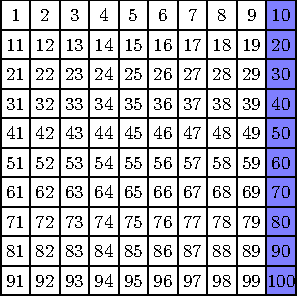
\includegraphics{10} \qquad \qquad
	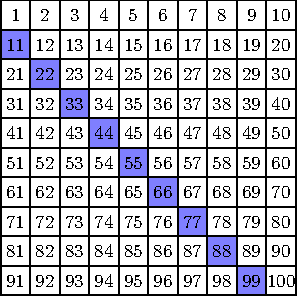
\includegraphics{11}
\end{center}
\end{document}